% Metódy inžinierskej práce — Prezentácia projektu
% Tím: M. Nosenko, V. Nedoluha, D. Nikolenko, R. Mykytiuk
% Preklad: latexmk -pdf prezentacia.tex  (alebo pdflatex + bibtex + pdflatex 2x)

\documentclass[10pt]{beamer}

% Téma a farebnosť — podľa cvičenia c06 možno meniť \usetheme a \usecolortheme:
%\usetheme{Warsaw}
%\usetheme{JuanLesPins}
%\usetheme{Goettingen}
%\usetheme{Boadilla}
\usetheme{Madrid}
%\usecolortheme{seahorse}
%\usecolortheme{rose}
%\usecolortheme{beaver}
\usecolortheme{dolphin}

\setbeamercovered{transparent}
\setbeamertemplate{navigation symbols}{}
\setbeamertemplate{footline}[frame number]

% shorthands=off: kvóty "..." v slovenčine inak rozbijú čítanie súboru .toc pri \tableofcontents
\usepackage[slovak,shorthands=off]{babel}
\usepackage[T1]{fontenc}
\usepackage[utf8]{inputenc}
\usepackage{lmodern}
\usepackage{url}
\usepackage{graphicx}
\usepackage{booktabs}
\graphicspath{{img/}}

% skrátenia podľa šablóny prez.tex (cvičenie c06)
\newcommand{\zdroj}[1]{\footnote{\tiny #1}}
\newcommand{\emp}[1]{\textit{\alert{#1}}}
\newcommand{\kw}[1]{\mbox{\textbf{#1}}}

\title[FAKERADAR]{Detekcia falošných online recenzií na základe jazykových a behaviorálnych príznakov}
\subtitle{Prezentácia projektu \textbf{FAKERADAR}\\
{\small Semestrálny projekt v predmete Metódy inžinierskej práce, ak. rok 2026/27}}
\author[Nosenko, Nedoluha, Nikolenko, Mykytiuk]{Matvii Nosenko, Volodymyr Nedoluha,\\ Danylo Nikolenko, Rostyslav Mykytiuk}
\institute{Fakulta informatiky a informačných technológií\\
Slovenská technická univerzita v Bratislave\\
{\small Vedenie projektu: Ing. Ivan Kapustík}}
\date{\footnotesize prezentácia projektu \textbullet\ zimný semester 2026/27}

\begin{document}

% ---------------------------------------------------------------
\begin{frame}
  \titlepage
  \begin{center}
    
\includegraphics[height=9mm]{STU-FIIT-nfv}
  \end{center}
\end{frame}

% ---------------------------------------------------------------
\begin{frame}{Motivácia}
\begin{itemize}
\item Online recenzie ovplyvňujú \kw{predaj, reputáciu aj rozhodovanie} spotrebiteľov
  \zdroj{Luca a Zervas, Management Science 2016}
\item Falošné recenzie vytvárajú firmy, platení recenzenti, konkurencia aj \kw{automatizované nástroje}
\item V ére veľkých jazykových modelov (LLM) je vymyslený text \emp{plynulý a lacný} --- povrchové detektory strácajú spoľahlivosť
  \zdroj{Zhao a kol., J. Retailing Consum. Serv. 2025}
\item Potrebné je \kw{ hybridné } riešenie: jazykové + behaviorálne príznaky, grafy a \emp{vysvetliteľný} výstup pre moderátora
\end{itemize}
\vfill
\begin{block}{Cieľ projektu FAKERADAR}
Navrhnúť a overiť modulárny, vysvetliteľný hybridný detektor falošných recenzií
vrátane prvej dvojjazyčnej (slovensko-anglickej) dátovej sady.
\end{block}
\end{frame}

% ---------------------------------------------------------------
\begin{frame}{Prehľad}
\tableofcontents
\end{frame}

% ---------------------------------------------------------------
\section{Úvod a ciele projektu}
\begin{frame}[plain]
  \centering
  {\LARGE\bfseries Úvod a ciele projektu}\\[3mm]
  {\large prednáša: \kw{Matvii Nosenko}}
\end{frame}

\begin{frame}{Výskumné otázky a ciele}
\begin{itemize}
\item \kw{RQ1:} Ktoré jazykové príznaky sú spojené s falošnými recenziami?
\item \kw{RQ2:} Ktoré behaviorálne a grafové príznaky zachytávajú koordinované podvody?
\item \kw{RQ3:} Ako tieto skupiny príznakov \emp{kombinovať} (early/late fusion)?
\item \kw{RQ4:} Ktoré problémy zostávajú otvorené v ére generatívnych modelov?
\item Ciele projektu
  \begin{itemize}
  \item dvojjazyčná anotovaná dátová sada recenzií
  \item porovnanie jazykových a behaviorálnych príznakov v podmienkach LLM
  \item hybridný detektor s vysvetliteľnými výstupmi
  \end{itemize}
\item Primárne usmernenie: prehľad Crawford a kol. 2015; zakladajúca práca oblasti: Jindal a Liu 2008
\end{itemize}
\end{frame}

% ---------------------------------------------------------------
\section{Súčasný stav v oblasti}
\begin{frame}[plain]
  \centering
  {\LARGE\bfseries Súčasný stav v oblasti}\\[3mm]
  {\large prednáša: \kw{Volodymyr Nedoluha}}
\end{frame}

\begin{frame}{Taxonómia recenzného spamu a súvisiace práce}
\begin{itemize}
\item Delenie podľa Jindala a Liua (2008):
  \begin{itemize}
  \item \emp{nepravdivé} recenzie, recenzie propagujúce značku, nerecenzie produktu
  \end{itemize}
\item Prvý štandardizovaný dataset a n-gramové detektory: Ott a kol. (2011)
\item Behaviorálne príznaky môžu byť \kw{informatívnejšie} než samotný text: Mukherjee a kol. (2013)
\item Koordinované skupiny a siete: Mukherjee a kol. (2012), Rayana a Akoglu (2015)
\item Prehľady a pravidlá zovšeobecňujúce datasety: Crawford a kol. (2015), Heydari a kol. (2015), Li a kol. (2014)
\item Aplikačný rámec pre spotrebnú elektroniku: Barbado a kol. (2019)
\end{itemize}
\vfill
{\tiny Zdroje: plný zoznam na poslednom slajde; článok odkazuje na 12+ zdrojov cez BibTeX.}
\end{frame}

\begin{frame}{Jazykové príznaky}
\begin{itemize}
\item \kw{Lexikálna bohatosť:} Type-Token Ratio (normalizovaný), dĺžka slova, slovná zásoba
  \zdroj{Ott a kol. 2011; Heydari a kol. 2015}
\item \kw{Syntax a slovné druhy:} falošné recenzie $\rightarrow$ viac slovies, prísloviek a zámen; reálne $\rightarrow$ viac podstatných mien
\item \kw{Sémantika a sentiment:} extrémne hodnotenie, málo overiteľných detailov
  \zdroj{Li a kol. 2014}
\item \kw{Neurónové reprezentácie:} jemne doladené transformery (BERT) + perplexita generovaných textov
  \zdroj{Devlin a kol. 2019; Zhao a kol. 2025}
\item Výhody: lacné, dostupné pri novom recenzentovi, interpretovateľné
\item Riziko: \emp{učenie sa idiosynkrázií} autorov/modelov $\Rightarrow$ slaba generalizácia
\end{itemize}
\end{frame}

\begin{frame}{Behaviorálne a grafové príznaky}
\begin{itemize}
\item \kw{Recenzent:} vek účtu, pomer recenzií k nákupom, podiel extrémnych hodnotení
\item \kw{Recenzia a produkt:} duplicitný text, odchýlka od priemeru, náhle zmeny ratingu
\item \kw{Čas:} burstiness, periodicita, synchronizácia účtov (burstové kampane)
\item \kw{Graf:} bipartitný graf recenzent--produkt, ko-recenzné skupiny, šírenie podozrenia
  \zdroj{Mukherjee a kol. 2012; Rayana a Akoglu 2015}
\end{itemize}
\begin{block}{Dôveryhodnosť recenzenta ako exponenciálne vyhladzovanie}
\[ T_n(u) = \alpha\,\phi\bigl(r_n(u)\bigr) + (1-\alpha)\,T_{n-1}(u), \qquad \alpha \in (0,1) \]
$\phi \in \langle 0,1\rangle$ --- normalizovaný signál autentickosti $n$-tej recenzie
\end{block}
{\tiny Obmedzenia: studený štart nových recenzentov, dostupnosť dát a GDPR.}
\end{frame}

\begin{frame}{Diagram: proces detekcie a architektúra extrakcie príznakov}
\begin{columns}
\begin{column}{0.44\textwidth}
  \centering
  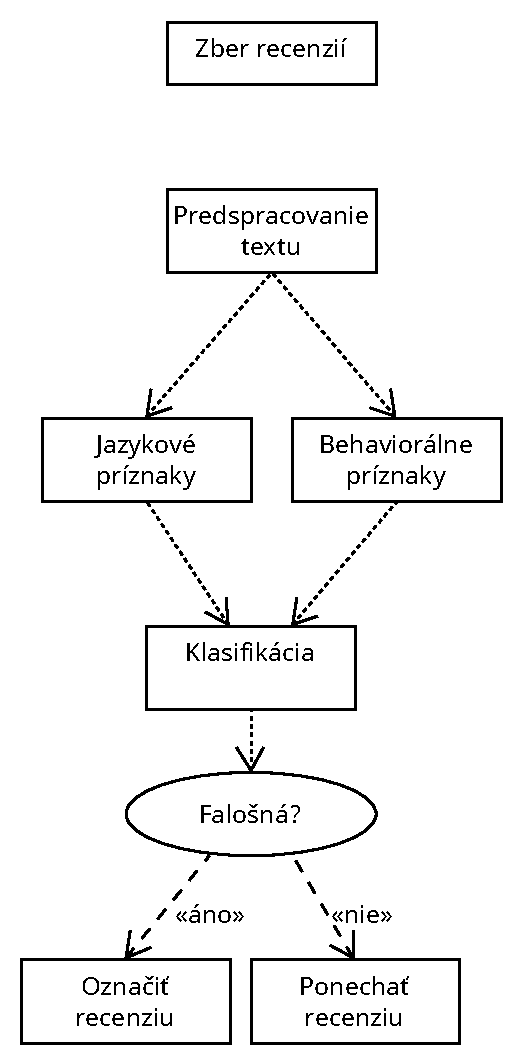
\includegraphics[width=\linewidth,height=0.72\textheight,keepaspectratio]{diagram1.pdf}
  \tiny Proces detekcie recenzií
\end{column}
\begin{column}{0.54\textwidth}
  \centering
  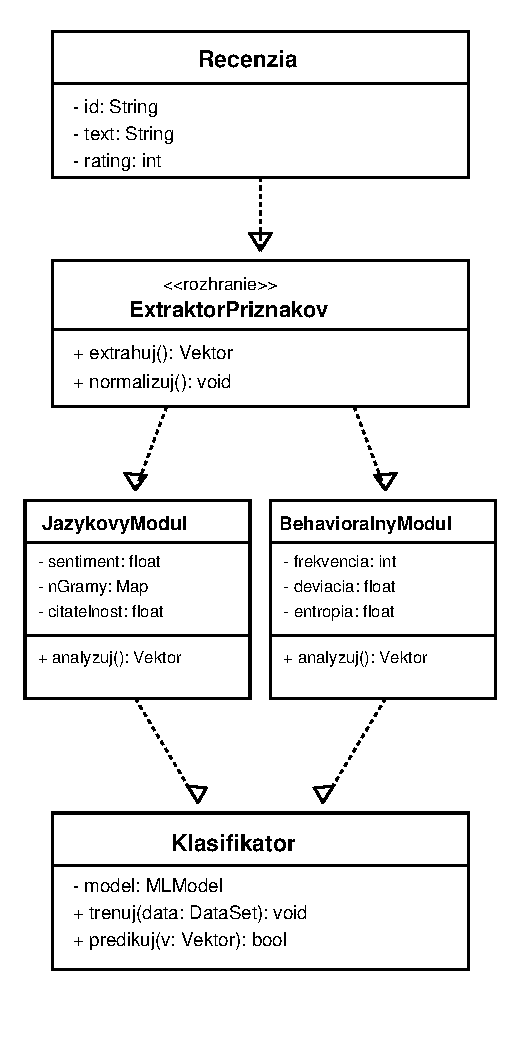
\includegraphics[width=\linewidth,height=0.72\textheight,keepaspectratio]{diagram2.pdf}
  \tiny Architektúra tried extraktora príznakov
\end{column}
\end{columns}
\vfill
{\tiny Diagramy vytvorené v nástroji \kw{UMLet} (zdrojové súbory: \texttt{img/diagram1.uxf}, \texttt{img/diagram2.uxf}).}
\end{frame}

% ---------------------------------------------------------------
\section{Porovnanie prístupov}
\begin{frame}[plain]
  \centering
  {\LARGE\bfseries Porovnanie prístupov}\\[3mm]
  {\large prednáša: \kw{Danylo Nikolenko}}
\end{frame}

\begin{frame}{Hybridné prístupy a výzva LLM}
\begin{itemize}
\item Kombinácia príznakových skupín: \kw{early fusion} (úroveň príznakov) alebo \kw{late fusion} (úroveň rozhodnutí)
\item Osvedčené modely: gradientové boosting stromy, ansámble, \emp{grafové neurónové siete} \zdroj{Rayana a Akoglu 2015}
\item Grafy šíria podozrenie na susedov $\Rightarrow$ odhalia \kw{kampane neviditeľné na úrovni jednej recenzie}
\item \kw{Vysvetliteľnosť} ako rovnocenný cieľ: moderátor musí rozhodnutie obhájiť --- SHAP/LIME, pozornosť, protifaktuály \zdroj{Lundberg a Lee 2017}
\item LLM-generované recenzie: plynulé a konzistentné $\Rightarrow$ lexikálne príznaky strácajú silu \zdroj{Zhao a kol. 2025}
\item Evaluácia: časové/doménové rozdelenie dát, F1, AUROC, falošné pozitíva pri fixnom zachytení, kalibrácia
\end{itemize}
\end{frame}

\begin{frame}{Porovnanie skupín prístupov}
\begin{table}
\centering
\resizebox{\textwidth}{!}{%
\begin{tabular}{@{}p{2.0cm}p{3.6cm}p{3.4cm}p{3.4cm}@{}}
\toprule
Prístup & Typické príznaky & Silné stránky & Obmedzenia \\
\midrule
Jazykový & n-gramy, TTR, slovné druhy, sentiment, perplexita & dostupný pri novom recenzentovi; interpretovateľný; lacný & závislý od jazyka a domény; zlyháva pri LLM \\
Behaviorálny & vek účtu, frekvencia, burstiness, odchýlka ratingu & odolný voči štylistickým úpravám; zachytáva koordináciu & studený štart; GDPR a dostupnosť dát \\
Grafový & bipartitné grafy, ko-recenzné skupiny, šírenie podozrenia & odhaľuje skupiny a kampane & náročný na dáta a výpočet; horšia vysvetliteľnosť \\
Hybridný & spojenie textových, behaviorálnych a grafových príznakov & najlepšia presnosť a robustnosť & zložitosť; riziko preučenia; náročná údržba \\
LLM-orientovaný & detekcia generovaného textu, adversariálne testovanie & reaguje na novú hrozbu & rýchly vývoj modelov; neistá generalizácia \\
\bottomrule
\end{tabular}}
\caption{Porovnanie skupín príznakov a prístupov k detekcii falošných recenzií.}
\end{table}
\end{frame}

\begin{frame}{Vážené vyhodnotenie prístupov (tabuľka z Excelu)}
\begin{table}
\centering
\footnotesize
\setlength{\tabcolsep}{4.5pt}
\begin{tabular}{@{}lccccc@{}}
\toprule
Kritérium (skóre 1--5) & Váha & Jazyk. & Behav. & Graf. & Hybrid. \\
\midrule
Presnosť v rámci domény           & 0{,}25 & 3 & 3 & 4 & \textbf{5} \\
Odolnosť voči LLM-generovaným textom & 0{,}20 & 1 & 4 & 3 & \textbf{4} \\
Zachytenie koordinovaných kampaní & 0{,}15 & 1 & 4 & 5 & \textbf{5} \\
Interpretovateľnosť výstupu       & 0{,}20 & \textbf{5} & 3 & 2 & 4 \\
Dostupnosť dát pri štarte         & 0{,}10 & \textbf{5} & 2 & 1 & 3 \\
Škálovateľnosť a náklady          & 0{,}10 & \textbf{4} & 3 & 2 & 3 \\
\midrule
\textbf{Vážené skóre (vzorec)}    & 1{,}00 & 3{,}00 & 3{,}25 & 3{,}05 & \textbf{4{,}20} \\
\bottomrule
\end{tabular}
\caption{Multikritériálne vyhodnotenie prístupov.}
\end{table}
\vfill
{\tiny Tabuľka spracovaná v LibreOffice Calc: \texttt{tabulky/tabulky\_fakeradar.xlsx}, list „Vyhodnotenie“;\\
posledný riadok počíta funkcia \texttt{=SUMPRODUCT(váhy; skóre)}, váhy overuje \texttt{=SUM(...)}\,=\,1.}
\end{frame}

% ---------------------------------------------------------------
\section{Navrhovaný prístup a plán}
\begin{frame}[plain]
  \centering
  {\LARGE\bfseries Navrhovaný prístup a plán}\\[3mm]
  {\large prednáša: \kw{Rostyslav Mykytiuk}}
\end{frame}

\begin{frame}{FAKERADAR: modulárny hybridný detektor}
\begin{columns}
\begin{column}{0.52\textwidth}
\begin{itemize}
\item \kw{1. Zber a anotácia dát} --- dvojjazyčná sada, medzanotátorská zhoda
\item \kw{2. Extrakcia príznakov} --- jazykové (text) + behaviorálne a grafové (správanie)
\item \kw{3. Hybridný klasifikátor} --- early/late fusion + grafové príznaky
\item \kw{4. Vrstva vysvetlenia} --- atribúcie príznakov pre moderátora
\end{itemize}
\end{column}
\begin{column}{0.46\textwidth}
  \centering
  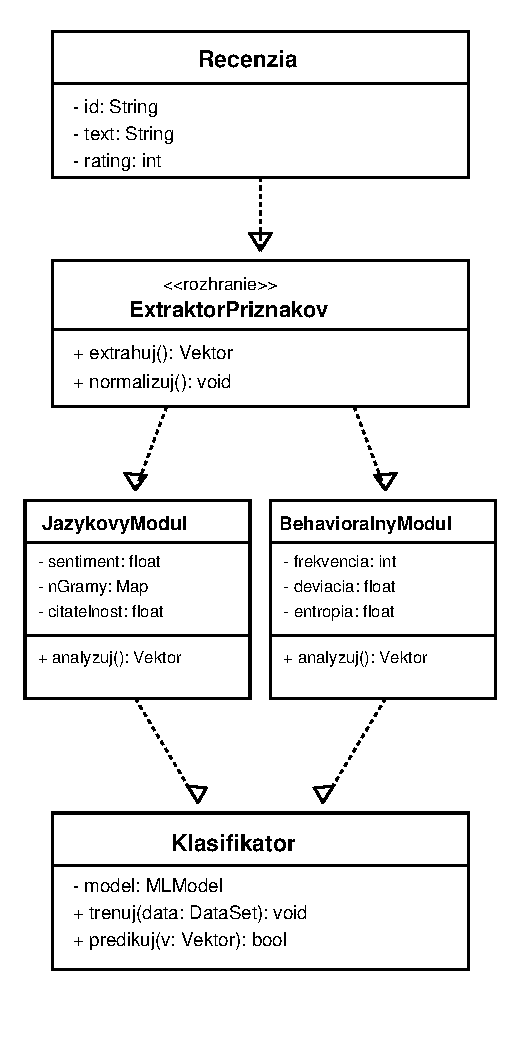
\includegraphics[width=\linewidth,height=0.74\textheight,keepaspectratio]{diagram2.pdf}
  \tiny Architektúra extraktora príznakov (UMLet)
\end{column}
\end{columns}
\end{frame}

\begin{frame}{Merateľné ciele a ukazovatele}
\begin{itemize}
\item \kw{Dátová sada:} 15\,000 anotovaných recenzií (sk/en), zhoda anotátorov $\kappa \geq 0{,}7$ \zdroj{Landis a Koch 1977}
\item \kw{Presnosť (F1, rámec domény):} jazykový model $\geq 0{,}80$; behaviorálny/grafový $\geq 0{,}75$; \emp{hybridný $\geq 0{,}85$}
\item \kw{Prenos na novú doménu:} F1 $\geq 0{,}75$; hodnotenie aj na časovo oddelených dátach (concept drift)
\item \kw{Hybridný model má prekonať} samostatné modely v porovnateľnom teste
\item \kw{Pilot:} s partnerskou platformou (pri dohode), inak offline test na dostupných dátach; latencia API sa meria
\item Kalibrácia prahov až po baseline experimentoch --- predbežné ciele sú pracovné, nie namerané
\end{itemize}
\end{frame}

\begin{frame}{Plán prác a rozdelenie v tíme}
\begin{table}
\centering
\footnotesize
\begin{tabular}{@{}lllc@{}}
\toprule
 & Pracovný balík & Obdobie (mes.) & Vedúci WP \\
\midrule
WP1 & manažment, reporting a riadenie rizík & 1--36 & M. Nosenko \\
WP2 & zber, anotácia a sprístupnenie dát & 1--12 & V. Nedoluha \\
WP3 & jazykové modely a baseline experimenty & 7--18 & M. Nosenko \\
WP4 & behaviorálne a grafové modely & 13--24 & V. Nedoluha \\
WP5 & hybridný model, fúzia a vrstva vysvetliteľnosti & 19--30 & D. Nikolenko \\
WP6 & pilotné overenie, prototyp API a evaluácia & 25--36 & R. Mykytiuk \\
WP7 & diseminácia, dokumentácia a publikácie & 1--36 & R. Mykytiuk \\
\bottomrule
\end{tabular}
\caption{Sedem pracovných balíkov projektu (zodpovedá formuláru VV-F a článku; detailná kapacitná tabuľka po hodinách: \texttt{tabulky/tabulky\_fakeradar.xlsx}, list „Harmonogram“, medzisúčty po riešiteľoch cez \texttt{=SUMIF}). Obdobie = mesiace od začiatku projektu (01/2027).}
\end{table}
\begin{itemize}
\item Zodpovednosť za balíky kopíruje odborné špecializácie tímu a spresní sa pri štarte projektu
\item Iteračný a inkrementálny postup: šprinty v Jira, revízie v Git-e
\end{itemize}
\end{frame}

% ---------------------------------------------------------------
\section*{Zhodnotenie a ďalšia práca}
\begin{frame}{Zhodnotenie a ďalšia práca}
\begin{itemize}
\item Jazykové príznaky = lacná \kw{prvotná filtrácia}; behaviorálne a grafové odhaľujú \kw{koordinované kampane}
\item Ťažisko výskumu sa posúva k \kw{hybridným riešeniam} s vysvetliteľnými výstupmi
\item Otvorené problémy: slovenské/české dáta, studený štart, posun distribúcie, adversariálne prispôsobovanie
\item Ďalšia práca: baseline experimenty na verejných datasetoch, tvorba dvojjazyčnej sady, kalibrácia cieľových hodnôt
\end{itemize}
\end{frame}

\begin{frame}{Otázky na diskusiu}
\begin{enumerate}
\item Má zmysel \emp{zakázať} AI-generované recenzie, alebo ich iba \emp{transparentne označovať}?
\item Ktorý kompromis preferuje moderátor: vyššia presnosť modelu alebo lepšia \emp{vysvetliteľnosť} rozhodnutia?
\item Ako zachytiť podvod \kw{v čase studeného štartu}, keď recenzent nemá žiadnu históriu?
\item Sú behaviorálne príznaky udržateľné vzhľadom na \emp{GDPR} a súkromie používateľov?
\end{enumerate}
\vfill
\begin{center}
{\Large \textbf{Ďakujeme za pozornosť!}}\\[1mm]
{\small Otázky radi zodpovieme --- diskutovať budú všetci členovia tímu.}
\end{center}
\end{frame}

% ---------------------------------------------------------------
\begin{frame}[allowframebreaks]{Zdroje}
\scriptsize
\setbeamertemplate{bibliography item}[text]
% celá bibliografia z .bib (textové odkazy na zdroje sú v nohách slajdov)
\nocite{*}
\bibliographystyle{unsrt}
\bibliography{literatura}
\end{frame}

\end{document}
